\section{Experiment and results}
In this chapter, Dynamic Correlated Topic Model(DCTM)\cite{tomasi_stochastic_nodate}, and Dynamic Embedded Topic Model(DETM)\cite{dieng_dynamic_2019} to compare with our model.\footnote{DTM was tested in our experiment, nonetheless, did not yield result after 10 hours of running time.}
\subsection{Experiment settings}
\paragraph{Datasets}
% First datasets, vocabularies, years 
We select the \textsc{un debates} as one of the testing corpus for the experiment. It is a collection of transcript from the official of UN member countries expressing about the  government's perspective over the world issues at the time.
After preprocessing, It contains 46 years time span of data, with 7507 documents and 6831 tokens in total. We selected 6005 for training, 1402 documents for testing and 100 documents for validation.
% Second datasets - NeurIPS 1987-2019
Second dataset we selected is \textsc{NeurIPS} conference paper dataset. The dataset contains conference papers ranged from 1987-2019. After preprocessing, it contains 9677 papers in total and 9182 tokens. Within the dataset, we pick 7345 documents for training, 1737 for testing and 100 for validation.
\paragraph{Data pre-processing}
To prepare the datasets for training, we pre-process the documents and turn them into useful corpus.
% Preprocess
We remove the special characters and stop words, and perform tokenization to split document sentences into a list of tokens. 
% three datas
In order to train the model, we have to leverage the datasets to feed-in different model. Specifically, the data are shaped into different forms.
% document-vocabularies
First, the bag-of-word $ w_{1:D}\in\mathbb{R}^{D\times V} $ is a matrix consist of the word count for vocabularies exist in every document. The document frequency for tokens are set to 100 documents minimum and 50\% at max.
% time-vocabularies
We also created a time-vocabularies word count matrix for the training of $ \eta $. The dataset $ \tilde{w}_{1:T}\in\mathbb{R}^{T\times V} $ holds the word count for the vocabulary set over the time span $ t=1,\dots,T $.
\paragraph{Transformer learning task}
% word sequence (seqlen=40) <OOV> <MASK> <IGNORE>
For transformer embedding training, we shape the dataset into a sequence set $ S $ of equal distance of pre-defined sentence length $ \textsc{seqlen} $. Token $ \textsc{<pad>} $ are padded to the sequence when the sentence in i-index $ S[i]\textsc{<seqlen>} $. The out-of-vocab tokens are replaced with $ \textsc{<oov>} $ token. The sequence dataset are to train the transformer embedding as input in the training process. To organize the training task, we define a set of token and target to Transformer learn it explicitly. We configure 15\% of tokens within a sentence are to be masked for the training task. First we replace a $ \textsc{<mask>} $ token on the selected word position of the token input. Other tokens will be filled a $ \textsc{<ignore>} $ token on the corresponding target position to exclude those token position to be calculate in the prediction score. 
% DTM, DETM, our model
\paragraph{Models}
% TODO
We maintain the default settings for DCTM \cite{tomasi_stochastic_nodate}, with 0.1 kernel bandwidth and 1 for kernel amplitude.\footnote{\url{https://github.com/spotify-research/dctm/}}
For D-ETM model, we follow the default settings instructed in \cite{dieng_dynamic_2019}. We set the variance of  on the prior to 0.005.\footnote{\url{https://github.com/adjidieng/DETM/}}
\paragraph{Algorithm configurations}
% alpha	
Following the parameter settings from \cite{blei_dynamic_2006}, the variance of prior in $  $ are set to $ \xi^2=0.005 $ on $ \alpha\sim\mathcal{N}(\cdot,\cdot) $.
% transformer
We set the dimension for the transformer embedding is 256, and so for the hidden dimension for both transformer encoder and decoder. Each transformer encoder and transformer decoder consist of two layers and 2 heads for scaled dot-product. The sequence length the transformer are set to 20.
% gaussian process
For the gaussian process latent variable model, we selected zero mean with squared exponential function (RBF kernel) as the covariance prior, which allows providing adaptive change on topic-proportion against the possible rapid topic changes from documents. The number of inducing point are set to 50. We follow the setting from \cite{tomasi_stochastic_nodate} and set the length scale of kernel as 0.1.
\subsection{Results}
\paragraph{Training}
In the training stage, we perform black box variational inference to estimate the unbiased gradient estimator with Monte Carlo sampling for intractable variational lower bound.
\paragraph{Quantitative results}
The result of models are to compare in terms of perplexity, Topic Coherence (TC), Topic Diversity (TD). To calculate the topic coherence and topic diversity, we average down the scores over time span $ 1\dots T $. We put the models into UN debates and NIPS dataset for comparison.

% non-time series
In addition to both of the results above, we also put the model we construct from chapter $ \ref{ch4} $ to compare with the time-series version models in this chapter. Since the model does not consider time series information, it only predicts a single set of topic words and thus for the TC and TD score.
% table for perplexity, topic coherence, and topic diversity
\begin{table}[h]
\centering
\begin{tabular}{llll}
\hline
     & Perplexity  &TC&TD\\ \hline
DCTM	     	&  4205.1 & -0.017 & \textbf{0.953}\\
D-ETM	     	&  \textbf{2842.1} & 0.076 & 0.427 \\
Our model(ch3) & 2746.3 & 0.152 & 0.643 \\
\textbf{Our model}  & 4103.8 & \textbf{0.092} & 0.429 \\ \hline
\end{tabular}
\captionof{table}{Result on UN debates dataset, k=30\label{tbl:ch6_t1}}
\end{table}
\begin{table}[h]
\centering
\begin{tabular}{llll}
\hline
     & Perplexity & TC & TD \\\hline
DCTM	     	& 4898.4 & -0.092 & \textbf{0.966} \\
D-ETM	     	& \textbf{2282.3} & 0.120 & 0.517 \\
Our model(ch3) & 1960.8 & 0.201 & 0.733 \\
\textbf{Our model}  & 5461.0 & \textbf{0.136} & 0.502 \\\hline
\end{tabular}
\captionof{table}{Result on NeurIPS dataset (1987-2019), k=30\label{tbl:ch6_t2}}
\end{table}

% model
From table \ref{tbl:ch6_t1}, we have compared our model with the latest model. We only highlight the times-series model with the highest score. 
% un debates
On the UN debate dataset, we conduct the experiment with number of topic $ k=30 $. In terms of perplexity, the D-ETM model has performed a better score. On the other hand, our model obtain a better performance in terms of topic coherence and topic diversity, which is 0.092 and 0.429 respectively. In particular, UN debates dataset tends to contain more diversified topic mentions in different years and word usages by leaders from different countries. 
% DCTM
The DCTM holds the best topic diversity value, but the poor result in perplexity and topic coherence score make it meaningless.
% nips dataset
On NIPS dataset, table \ref{tbl:ch6_t2} contains the scores that we obtained from each model we conducted experiment. From the result, when $ k=30 $, our model resulted 0.136 in topic coherence score and 0.502 in topic diversity. To compare with other instances, our model perform the best in topic coherence score. D-ETM has the lowest perplexity score, which perform the best in predictive task. On the other hand, our model has apparently beats the other models in both TC and TD scores. 
\subsubsection{Qualitative results}
% visualization for the documents by topics
\paragraph{UN debates}We put the document-topic proportion obtained from the model and run t-SNE algorithm to transform the document-topic proportion into 2-dimensional continuous space. Shown in figure \ref{fig:tsne1}, different colors of dots represent a specific topic. As can be seen, apparently the documents can be classified in to interpretable cluster according to their topic.\\
\begin{figure}[h]
\centering
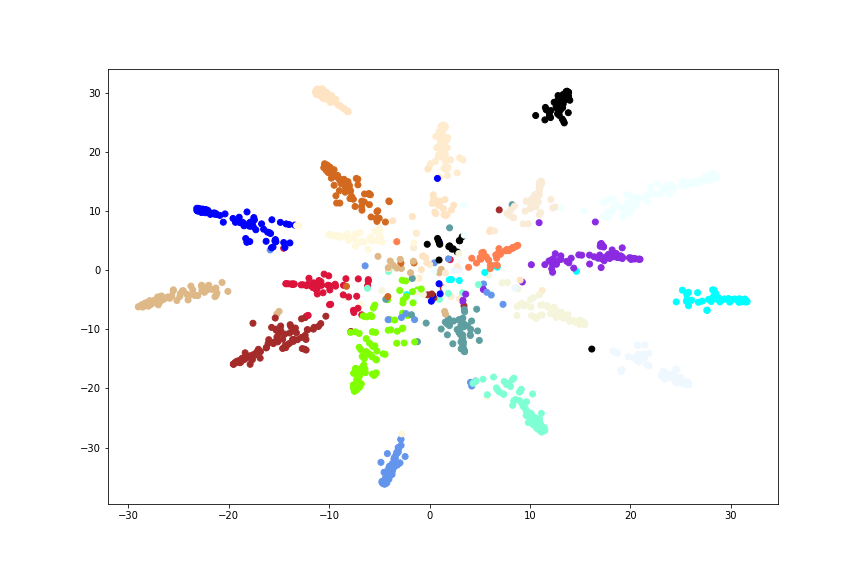
\includegraphics[width=0.9\linewidth]{figures/1128/tsne1}
\caption{t-SNE visualization for documents labeled by topic(UN debates)}
\label{fig:tsne1}
\end{figure}
% Scatter visualization for the words over time
From the result we obtained, we select top-6 topics have the highest proportion to the document set and display them on figure \ref{fig:scatter}. And for those topics, we extract top-5 words having the highest proportion. Then we track those words how they change their proportion to the corresponding topic. As demonstrated, the topic words in each topic selected doesn't diverse each other very much in proportion, resulted a coherent trend that the word are more likely adhere to the topic.\\
% add specific information, what can you see from the word on some topic
\begin{figure}[h]
\centering
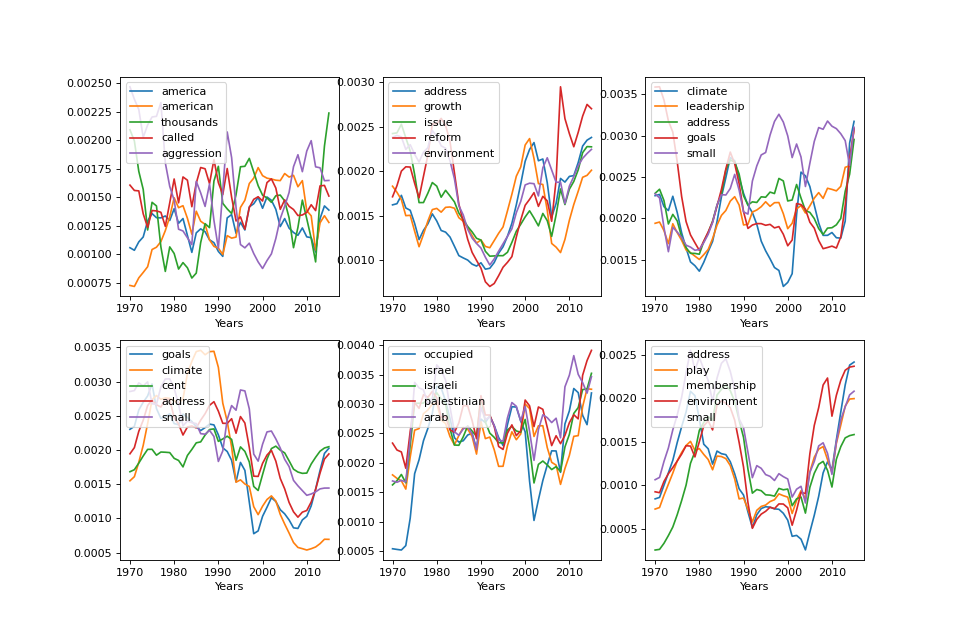
\includegraphics[width=0.9\linewidth]{figures/1220/scatter}
\caption{Word trend for top-6 topics (UN debates)}
\label{fig:scatter}
\end{figure}
% topic over time representation
Accordingly, in figure \ref{fig:stack} we also track the change of those topic over time. Different color in the cumulative graph represents the topics evolve along the time period. \\
% Specific: explain what you saw from the topic trend
\begin{figure}[h]
\centering
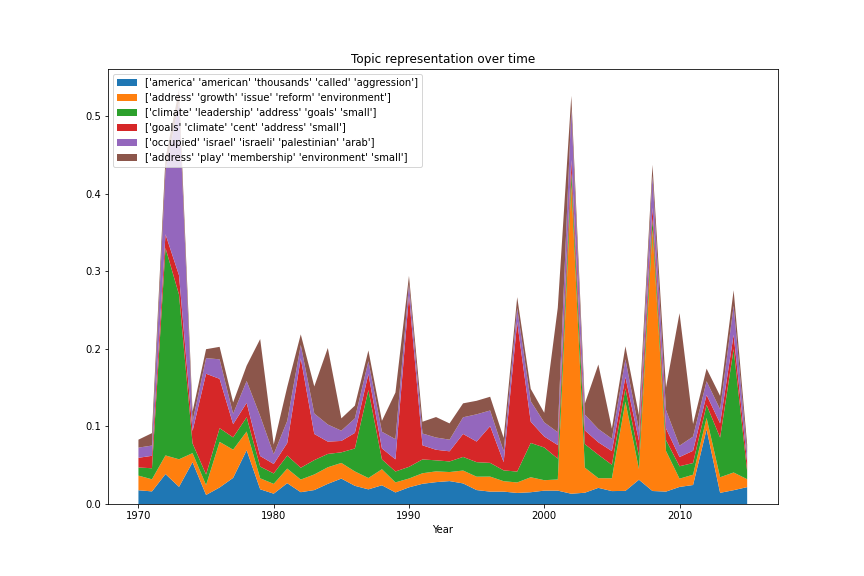
\includegraphics[width=0.9\linewidth]{figures/1220/stack}
\caption{Topic trend for top-6 topics (UN debate)}
\label{fig:stack}
\end{figure}
% NeurIPS
\paragraph{NeurIPS dataset} % we put k=20 into experiment setting
To investigate the word trends change over time, table \ref{tbl:ch6_t3} visualize the words by 5 years interval. In particular, we selected a topic corresponding to reinforcement learning and pick top-10 words for each time stamp. By observation, we see that the topic are coherent in several keywords like \textsc{control}, \textsc{action} and \textsc{state}. On the other hand, some other keywords also highlight their importance upon specific time period. For instance, words like \textsc{markov}, \textsc{policy} and \textsc{discount} are more likely to appear before; word \textsc{reinforcement} appears since 2012. For sake of interpretability, we also highlight the first appearance in the year for those keywords related to reinforcement learning.
% Figure word trend
On figure\ref{fig:scatter2}, displays the word trend from top-6 topics over the time. We have selected 3 representative tokens from top-10 words for each topic. And observe how the words trends though the years.
% Topic trend over time
On figure \ref{fig:stack2}, we provide a stack plot for how those top-6 topics changed over time. Apparently it demonstrates how the topics are inclining or declining. For example, the topic related to "reinforcement" is gaining more popularity over time. Besides, the topic about "cortex, cells" is being less important by the years.
\begin{figure}[h]
\centering
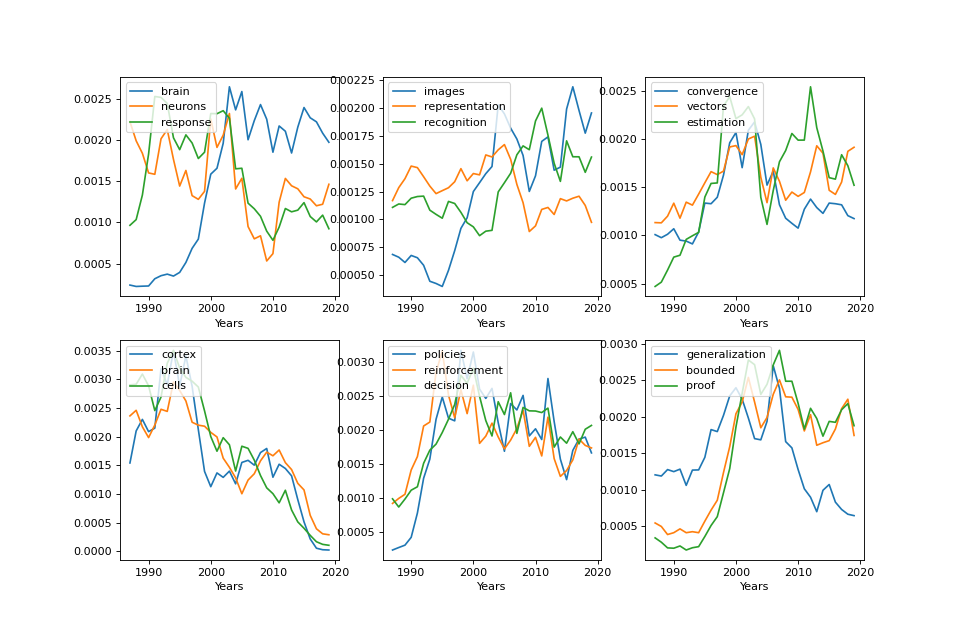
\includegraphics[width=1\linewidth]{figures/1128/scatter(2)}
\caption{Word trend for top-6 topics (NeurIPS dataset)}
\label{fig:scatter2}
\end{figure}
\begin{table}[h]
\centering
\begin{tabular}{ll}
\hline
Year&Topic: Reinforcement Learning\\ \hline
-&policy reward action goal control \\
&agent states actions reinforcement search\\
1987 &\hl{control} position world simulated initial \\
&search change \hl{environment} modification \hl{action}\\
1992 &temporal watkins cambridge dynamic controller \\
&sutton \hl{states} control actions action\\
1997 &states actions \hl{markov} \hl{decision} control \\
&dynamic \hl{discount} action discounted \hl{policy}\\
2002 &\hl{transition} decision dynamic \hl{reward} markov \\
&policies states actions policy action\\
2007 &artificial intelligence rewards policies programming \\
&states action reward actions policy\\
2012 &\hl{reinforcement} decision markov states mdp \\
&action policies reward actions policy\\
2017 &action markov policies reinforcement transition \\
&expected control states policy reward\\
\hline
\end{tabular}
\captionof{table}{Word trend in topic reinforcement learning (5 years interval)\label{tbl:ch6_t3}}
\end{table}
\begin{figure}[h]
\centering
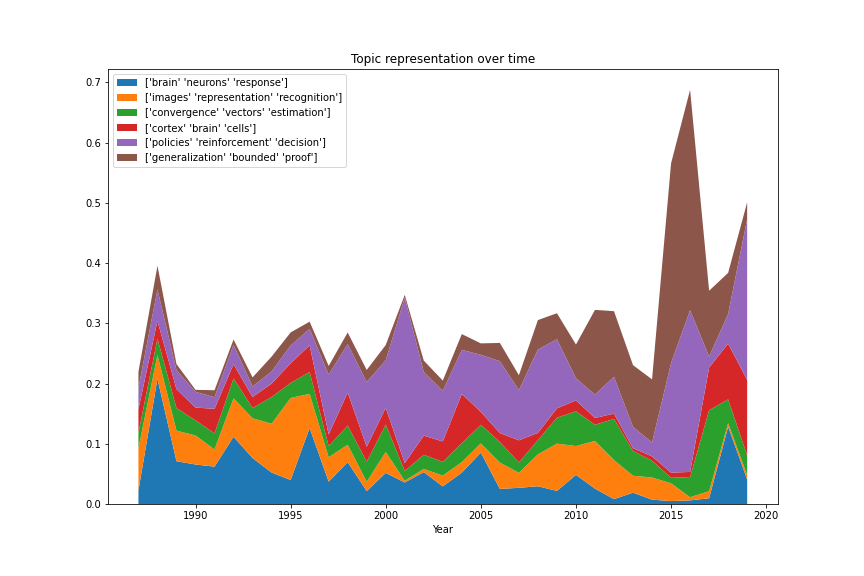
\includegraphics[width=1\linewidth]{figures/1128/stack(2)}
\caption{Topic trend for top-6 topics (NeurIPS dataset)}
\label{fig:stack2}
\end{figure}
% Discussion
\subsection{Discussion}
In the result, we observe that our model has been out perform the D-ETM model in TC and TD scores. Apparently the topic words in our model generated are both consistent  and coherent over time.
% the worse performance
On the other hand, we notice that our model does not beat the state-of-the-art model in perplexity. Which we speculate that the model trade off the loss from training transformer bring down the predictive performance of the model.
% Give observation
From analyzing the trend of the word and word group from each topic, we investigate how good the words obtain from each topic evolve over time. We convince that our model can obtain coherent topic from the document set and retrieve diverse keywords during the time span.